% ============================================================================
% UNIFY -- Diagram 5 (Haaniah)
% Sequence: ingestion with duplicate, out-of-order and missed-event handling
% Traces to proposal v2 sec. 8.3 (normalised envelope) and sec. 8.4 (reliability)
% Build: pdflatex 05_ingestion_sequence.tex
% ============================================================================
\documentclass[border=12pt]{standalone}
% =============================================================================
% UNIFY -- shared TikZ style used by Haaniah's self-contained diagrams
%          (05_ingestion_sequence.tex, 06_state_machines.tex, 11_deployment.tex)
%
% Those three files each start with \documentclass{standalone} + % =============================================================================
% UNIFY -- shared TikZ style used by Haaniah's self-contained diagrams
%          (05_ingestion_sequence.tex, 06_state_machines.tex, 11_deployment.tex)
%
% Those three files each start with \documentclass{standalone} + % =============================================================================
% UNIFY -- shared TikZ style used by Haaniah's self-contained diagrams
%          (05_ingestion_sequence.tex, 06_state_machines.tex, 11_deployment.tex)
%
% Those three files each start with \documentclass{standalone} + \input{unifystyle}
% and are compiled on their own ("pdflatex <file>.tex"), unlike Mishal's and
% Abdullah's sources, which are fragments wrapped by build.sh.
%
% The original unifystyle.tex was never committed. This file was reconstructed
% so the folder is self-contained again: the palette below was sampled directly
% from the committed renders (rendered/*.png, 200 dpi), and the geometry was
% matched against them. A rebuild should reproduce the committed PDFs closely;
% if you edit a style here, re-render all three and eyeball the diff.
%
% Layout note: like unify-diagram-styles.tex, this is plain TikZ (no tikz-uml),
% so it compiles in any TeX Live.
% =============================================================================
% Times, to match the report body and the fragment diagrams
\usepackage{mathptmx}
\usepackage[T1]{fontenc}
\usepackage{tikz}
\usepackage{pgffor} % \foreach (05_ingestion_sequence lifelines)
\usetikzlibrary{arrows.meta,positioning,calc,fit,backgrounds,
                shapes.geometric,shapes.multipart,decorations.pathreplacing}

% ---- palette: exact fills sampled from the committed renders ----------------
\definecolor{extgrey}{HTML}{EDEDED}    % vendor / superseded (neutral)
\definecolor{relblue}{HTML}{CFE2F3}    % pipeline steps, fresh path
\definecolor{graphgreen}{HTML}{D9EAD3} % evidence graph / applied
\definecolor{verorange}{HTML}{FCE5CD}  % verification / findings / model
\definecolor{badred}{HTML}{F8D7DA}     % rejected / SOURCE_STALE
\definecolor{okgreen}{HTML}{DFF0D8}    % discarded / ignored / resolved
\definecolor{warnamber}{HTML}{FCE8C3}  % degraded / disputed
\definecolor{hynote}{HTML}{FFF9D6}     % side-note boxes

\tikzset{
  % ---- 05: sequence diagram --------------------------------------------------
  lane/.style={draw, fill=#1, rounded corners=2pt, inner sep=4pt,
               align=center, font=\bfseries\scriptsize},
  frame/.style={draw},                       % sdframe rectangles
  ftab/.style={draw, fill=white, font=\scriptsize, inner sep=1.5pt}, % alt A tab
  msg/.style={-{Stealth[length=2.5mm]}},     % call arrow
  ret/.style={-{Stealth[length=2.5mm]}, dashed}, % return arrow
  box/.style={draw, fill=#1, rounded corners=2pt, inner sep=4pt, align=center},
  % ---- 06: state machines ----------------------------------------------------
  st/.style={draw, fill=#1, rounded corners=2pt, inner sep=4pt,
             align=center, font=\scriptsize},
  dec/.style={diamond, aspect=1.75, draw, fill=white, font=\scriptsize,
              align=center, text width=1.5cm, inner sep=1pt},
  tr/.style={-{Stealth[length=2.2mm]}},       % state transition
  % ---- shared ----------------------------------------------------------------
  lbl/.style={font=\scriptsize, fill=white, inner sep=1pt},
  mlbl/.style={font=\scriptsize, align=center, inner sep=1pt}, % message label, sits above the arrow
  note/.style={draw, fill=hynote, font=\scriptsize, align=left,
               text width=#1, inner sep=4pt, rounded corners=2pt},
  note/.default=4.6cm,
}

% and are compiled on their own ("pdflatex <file>.tex"), unlike Mishal's and
% Abdullah's sources, which are fragments wrapped by build.sh.
%
% The original unifystyle.tex was never committed. This file was reconstructed
% so the folder is self-contained again: the palette below was sampled directly
% from the committed renders (rendered/*.png, 200 dpi), and the geometry was
% matched against them. A rebuild should reproduce the committed PDFs closely;
% if you edit a style here, re-render all three and eyeball the diff.
%
% Layout note: like unify-diagram-styles.tex, this is plain TikZ (no tikz-uml),
% so it compiles in any TeX Live.
% =============================================================================
% Times, to match the report body and the fragment diagrams
\usepackage{mathptmx}
\usepackage[T1]{fontenc}
\usepackage{tikz}
\usepackage{pgffor} % \foreach (05_ingestion_sequence lifelines)
\usetikzlibrary{arrows.meta,positioning,calc,fit,backgrounds,
                shapes.geometric,shapes.multipart,decorations.pathreplacing}

% ---- palette: exact fills sampled from the committed renders ----------------
\definecolor{extgrey}{HTML}{EDEDED}    % vendor / superseded (neutral)
\definecolor{relblue}{HTML}{CFE2F3}    % pipeline steps, fresh path
\definecolor{graphgreen}{HTML}{D9EAD3} % evidence graph / applied
\definecolor{verorange}{HTML}{FCE5CD}  % verification / findings / model
\definecolor{badred}{HTML}{F8D7DA}     % rejected / SOURCE_STALE
\definecolor{okgreen}{HTML}{DFF0D8}    % discarded / ignored / resolved
\definecolor{warnamber}{HTML}{FCE8C3}  % degraded / disputed
\definecolor{hynote}{HTML}{FFF9D6}     % side-note boxes

\tikzset{
  % ---- 05: sequence diagram --------------------------------------------------
  lane/.style={draw, fill=#1, rounded corners=2pt, inner sep=4pt,
               align=center, font=\bfseries\scriptsize},
  frame/.style={draw},                       % sdframe rectangles
  ftab/.style={draw, fill=white, font=\scriptsize, inner sep=1.5pt}, % alt A tab
  msg/.style={-{Stealth[length=2.5mm]}},     % call arrow
  ret/.style={-{Stealth[length=2.5mm]}, dashed}, % return arrow
  box/.style={draw, fill=#1, rounded corners=2pt, inner sep=4pt, align=center},
  % ---- 06: state machines ----------------------------------------------------
  st/.style={draw, fill=#1, rounded corners=2pt, inner sep=4pt,
             align=center, font=\scriptsize},
  dec/.style={diamond, aspect=1.75, draw, fill=white, font=\scriptsize,
              align=center, text width=1.5cm, inner sep=1pt},
  tr/.style={-{Stealth[length=2.2mm]}},       % state transition
  % ---- shared ----------------------------------------------------------------
  lbl/.style={font=\scriptsize, fill=white, inner sep=1pt},
  mlbl/.style={font=\scriptsize, align=center, inner sep=1pt}, % message label, sits above the arrow
  note/.style={draw, fill=hynote, font=\scriptsize, align=left,
               text width=#1, inner sep=4pt, rounded corners=2pt},
  note/.default=4.6cm,
}

% and are compiled on their own ("pdflatex <file>.tex"), unlike Mishal's and
% Abdullah's sources, which are fragments wrapped by build.sh.
%
% The original unifystyle.tex was never committed. This file was reconstructed
% so the folder is self-contained again: the palette below was sampled directly
% from the committed renders (rendered/*.png, 200 dpi), and the geometry was
% matched against them. A rebuild should reproduce the committed PDFs closely;
% if you edit a style here, re-render all three and eyeball the diff.
%
% Layout note: like unify-diagram-styles.tex, this is plain TikZ (no tikz-uml),
% so it compiles in any TeX Live.
% =============================================================================
% Times, to match the report body and the fragment diagrams
\usepackage{mathptmx}
\usepackage[T1]{fontenc}
\usepackage{tikz}
\usepackage{pgffor} % \foreach (05_ingestion_sequence lifelines)
\usetikzlibrary{arrows.meta,positioning,calc,fit,backgrounds,
                shapes.geometric,shapes.multipart,decorations.pathreplacing}

% ---- palette: exact fills sampled from the committed renders ----------------
\definecolor{extgrey}{HTML}{EDEDED}    % vendor / superseded (neutral)
\definecolor{relblue}{HTML}{CFE2F3}    % pipeline steps, fresh path
\definecolor{graphgreen}{HTML}{D9EAD3} % evidence graph / applied
\definecolor{verorange}{HTML}{FCE5CD}  % verification / findings / model
\definecolor{badred}{HTML}{F8D7DA}     % rejected / SOURCE_STALE
\definecolor{okgreen}{HTML}{DFF0D8}    % discarded / ignored / resolved
\definecolor{warnamber}{HTML}{FCE8C3}  % degraded / disputed
\definecolor{hynote}{HTML}{FFF9D6}     % side-note boxes

\tikzset{
  % ---- 05: sequence diagram --------------------------------------------------
  lane/.style={draw, fill=#1, rounded corners=2pt, inner sep=4pt,
               align=center, font=\bfseries\scriptsize},
  frame/.style={draw},                       % sdframe rectangles
  ftab/.style={draw, fill=white, font=\scriptsize, inner sep=1.5pt}, % alt A tab
  msg/.style={-{Stealth[length=2.5mm]}},     % call arrow
  ret/.style={-{Stealth[length=2.5mm]}, dashed}, % return arrow
  box/.style={draw, fill=#1, rounded corners=2pt, inner sep=4pt, align=center},
  % ---- 06: state machines ----------------------------------------------------
  st/.style={draw, fill=#1, rounded corners=2pt, inner sep=4pt,
             align=center, font=\scriptsize},
  dec/.style={diamond, aspect=1.75, draw, fill=white, font=\scriptsize,
              align=center, text width=1.5cm, inner sep=1pt},
  tr/.style={-{Stealth[length=2.2mm]}},       % state transition
  % ---- shared ----------------------------------------------------------------
  lbl/.style={font=\scriptsize, fill=white, inner sep=1pt},
  mlbl/.style={font=\scriptsize, align=center, inner sep=1pt}, % message label, sits above the arrow
  note/.style={draw, fill=hynote, font=\scriptsize, align=left,
               text width=#1, inner sep=4pt, rounded corners=2pt},
  note/.default=4.6cm,
}


\begin{document}
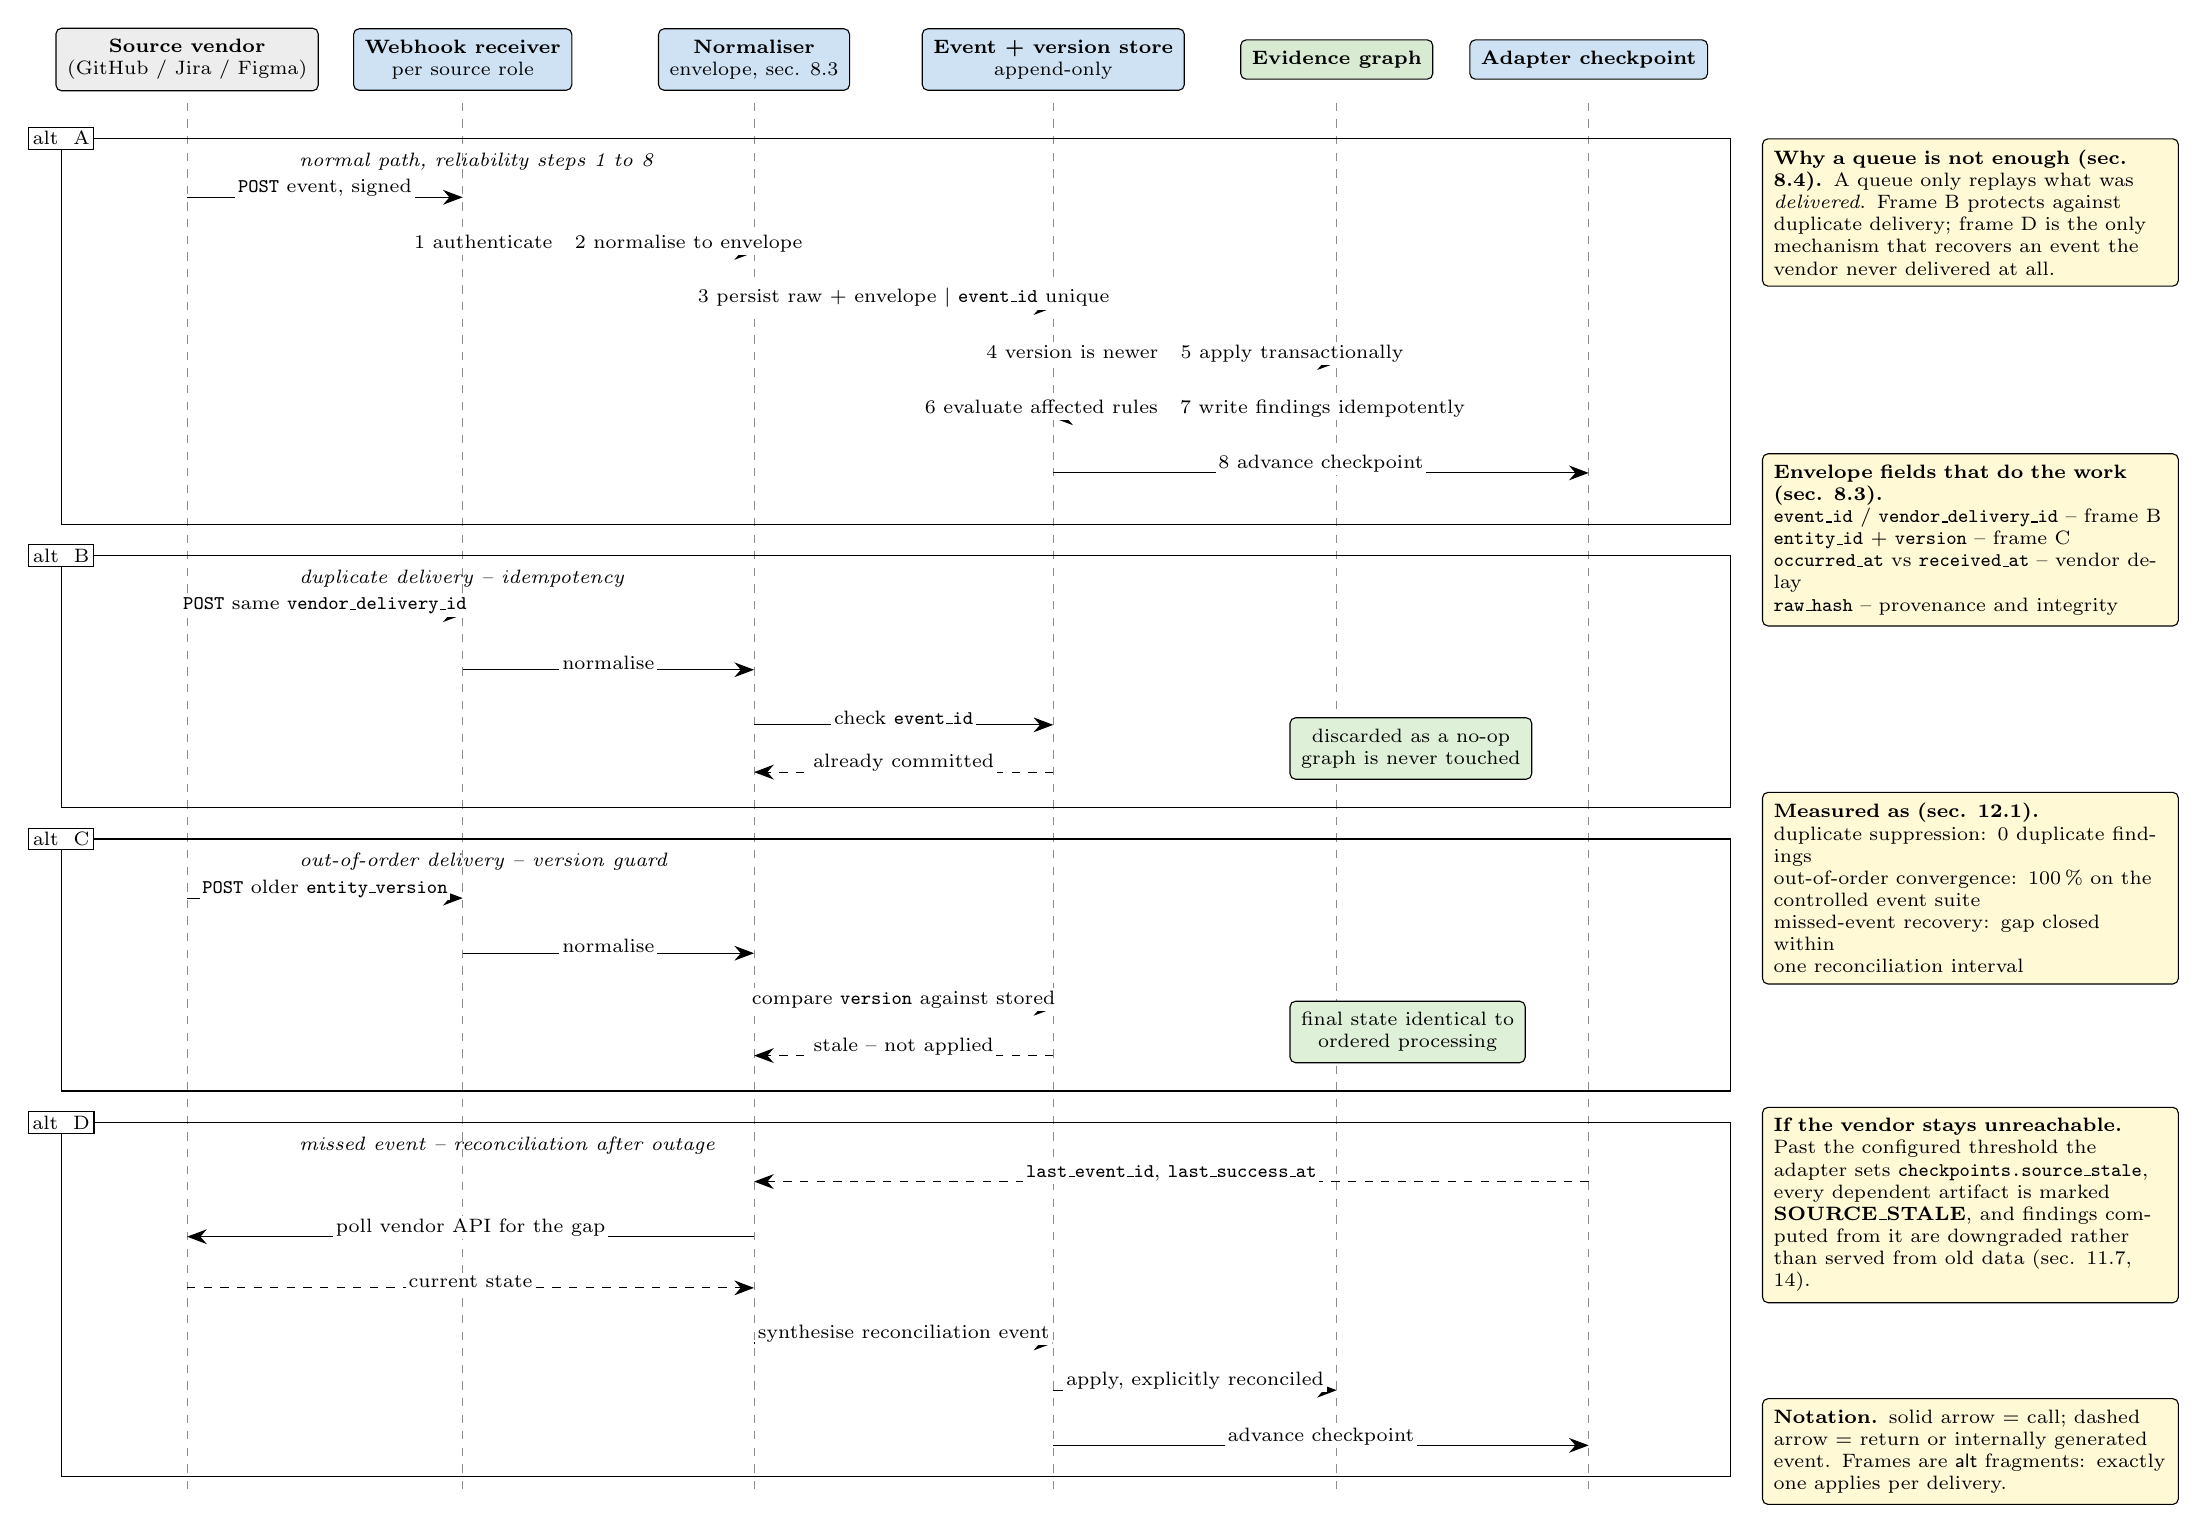
\begin{tikzpicture}[x=1cm,y=1cm]

% ---- lifelines ---------------------------------------------------------
\def\ybot{-18.2}
\foreach \x/\name/\col in {%
   0/{Source vendor\\\scriptsize\mdseries(GitHub / Jira / Figma)}/extgrey,
   3.5/{Webhook receiver\\\scriptsize\mdseries per source role}/relblue,
   7.2/{Normaliser\\\scriptsize\mdseries envelope, sec. 8.3}/relblue,
  11.0/{Event + version store\\\scriptsize\mdseries append-only}/relblue,
  14.6/{Evidence graph}/graphgreen,
  17.8/{Adapter checkpoint}/relblue}
  {
   \node[lane=\col] (L\x) at (\x,0) {\name};
   \draw[black!45,dashed] (\x,-0.55) -- (\x,\ybot);
  }

% ---- frame helper ------------------------------------------------------
\newcommand{\sdframe}[4]{% ytop, ybottom, tab, caption
  \draw[frame] (-1.6,#1) rectangle (19.6,#2);
  \node[ftab] at (-1.6,#1) {#3};
  \node[font=\scriptsize\itshape,anchor=north west] at (-1.6+2.9,#1-0.06) {#4};
}

% ========================= A. first delivery ============================
\sdframe{-1.0}{-5.9}{alt\ \ A}{normal path, reliability steps 1 to 8}

\draw[msg] (0,-1.75) -- node[lbl,pos=.5,above=-1pt]{\texttt{POST} event, signed} (3.5,-1.75);
\draw[msg] (3.5,-2.45) -- node[lbl,pos=.5,above=-1pt]{1 authenticate \ \ 2 normalise to envelope} (7.2,-2.45);
\draw[msg] (7.2,-3.15) -- node[lbl,pos=.5,above=-1pt]{3 persist raw + envelope \textbar\ \texttt{event\_id} unique} (11.0,-3.15);
\draw[msg] (11.0,-3.85) -- node[lbl,pos=.5,above=-1pt]{4 version is newer \ \ 5 apply transactionally} (14.6,-3.85);
\draw[ret] (14.6,-4.55) -- node[lbl,pos=.5,above=-1pt]{6 evaluate affected rules \ \ 7 write findings idempotently} (11.0,-4.55);
\draw[msg] (11.0,-5.25) -- node[lbl,pos=.5,above=-1pt]{8 advance checkpoint} (17.8,-5.25);

% ========================= B. duplicate =================================
\sdframe{-6.3}{-9.5}{alt\ \ B}{duplicate delivery -- idempotency}

\draw[msg] (0,-7.05) -- node[lbl,pos=.5,above=-1pt]{\texttt{POST} same \texttt{vendor\_delivery\_id}} (3.5,-7.05);
\draw[msg] (3.5,-7.75) -- node[lbl,pos=.5,above=-1pt]{normalise} (7.2,-7.75);
\draw[msg] (7.2,-8.45) -- node[lbl,pos=.5,above=-1pt]{check \texttt{event\_id}} (11.0,-8.45);
\draw[ret] (11.0,-9.05) -- node[lbl,pos=.5,above=-1pt]{already committed} (7.2,-9.05);
\node[box=okgreen,anchor=west,font=\scriptsize] at (14.0,-8.75)
  {discarded as a no-op\\graph is never touched};

% ========================= C. out of order ==============================
\sdframe{-9.9}{-13.1}{alt\ \ C}{out-of-order delivery -- version guard}

\draw[msg] (0,-10.65) -- node[lbl,pos=.5,above=-1pt]{\texttt{POST} older \texttt{entity\_version}} (3.5,-10.65);
\draw[msg] (3.5,-11.35) -- node[lbl,pos=.5,above=-1pt]{normalise} (7.2,-11.35);
\draw[msg] (7.2,-12.05) -- node[lbl,pos=.5,above=-1pt]{compare \texttt{version} against stored} (11.0,-12.05);
\draw[ret] (11.0,-12.65) -- node[lbl,pos=.5,above=-1pt]{stale -- not applied} (7.2,-12.65);
\node[box=okgreen,anchor=west,font=\scriptsize] at (14.0,-12.35)
  {final state identical to\\ordered processing};

% ========================= D. reconciliation ============================
\sdframe{-13.5}{-18.0}{alt\ \ D}{missed event -- reconciliation after outage}

\draw[ret] (17.8,-14.25) -- node[lbl,pos=.5,above=-1pt]{\texttt{last\_event\_id}, \texttt{last\_success\_at}} (7.2,-14.25);
\draw[msg] (7.2,-14.95) -- node[lbl,pos=.5,above=-1pt]{poll vendor API for the gap} (0,-14.95);
\draw[ret] (0,-15.6) -- node[lbl,pos=.5,above=-1pt]{current state} (7.2,-15.6);
\draw[msg] (7.2,-16.3) -- node[lbl,pos=.5,above=-1pt]{synthesise reconciliation event} (11.0,-16.3);
\draw[msg] (11.0,-16.9) -- node[lbl,pos=.5,above=-1pt]{apply, explicitly reconciled} (14.6,-16.9);
\draw[msg] (11.0,-17.6) -- node[lbl,pos=.5,above=-1pt]{advance checkpoint} (17.8,-17.6);

% ---- notes -------------------------------------------------------------
\node[note=5.0cm,anchor=north west] at (20.0,-1.0)
  {\textbf{Why a queue is not enough (sec. 8.4).}
   A queue only replays what was \emph{delivered}. Frame~B protects against
   duplicate delivery; frame~D is the only mechanism that recovers an event
   the vendor never delivered at all.};

\node[note=5.0cm,anchor=north west] at (20.0,-5.0)
  {\textbf{Envelope fields that do the work (sec. 8.3).}\\
   \texttt{event\_id} / \texttt{vendor\_delivery\_id} -- frame B\\
   \texttt{entity\_id} + \texttt{version} -- frame C\\
   \texttt{occurred\_at} vs \texttt{received\_at} -- vendor delay\\
   \texttt{raw\_hash} -- provenance and integrity};

\node[note=5.0cm,anchor=north west] at (20.0,-9.3)
  {\textbf{Measured as (sec. 12.1).}\\
   duplicate suppression: 0 duplicate findings\\
   out-of-order convergence: 100\,\% on the\\controlled event suite\\
   missed-event recovery: gap closed within\\one reconciliation interval};

\node[note=5.0cm,anchor=north west] at (20.0,-13.3)
  {\textbf{If the vendor stays unreachable.}
   Past the configured threshold the adapter sets
   \texttt{checkpoints.source\_stale}, every dependent artifact is marked
   \textbf{SOURCE\_STALE}, and findings computed from it are downgraded
   rather than served from old data (sec. 11.7, 14).};

% ---- legend ------------------------------------------------------------
\node[note=5.0cm,anchor=north west] at (20.0,-17.0)
  {\textbf{Notation.} solid arrow = call; dashed arrow = return or
   internally generated event. Frames are \textsf{alt} fragments: exactly one
   applies per delivery.};

\end{tikzpicture}
\end{document}
